% ------------------------------------------------------------------------------
% The implemtations shows specifically how your research was conducted.
% All the impementation details and practical tests can be listed.
% ------------------------------------------------------------------------------

\opt{never}{\addbibresource{03-tail/bibliography.bib}} % to make citation found in most IDE

\chapter{Implementation}
\label{chap:implementation}

% -- Your text goes here --
The implementation sets out the concrete realisation of the reference architecture, detailing the tools used to automate the deployment of the \gls{cloud_infrastructure} and the integration of the embedded systems. Particular attention is paid to the in-depth description of the automated pipeline. The various applications that accompany this architecture are also highlighted.

\minitoc
\newpage

% ------------------------------------------------------------------------------
\section{Reference architecture}

% -- Your text goes here --
\subsection{\Gls{cloud_infrastructure}}
An \acrfull{iac} tool was selected to orchestrate the efficient deployment of the \gls{cloud_infrastructure} on \gls{aws}, and Pulumi was chosen because of its choice of programming language, in this case Python. The use of the same programming language for the implementation of applications and the description of \gls{aws} resources provides consistency within the project.

Integrating Pulumi is simple. The resources required are described in Python files. The deployment is managed by the Pulumi \acrshort{cli}, which records the state of the infrastructure in an Amazon S3 compartment. This compartment is located in the same \gls{aws} account as the infrastructure, using Amazon S3 to store the state rather than the default Pulumi \Gls{cloud} platform, thus eliminating external dependencies. Figure \ref{fig:pulumi_overview} shows an overview of this part of the implementation.
\begin{center}
    \begingroup
    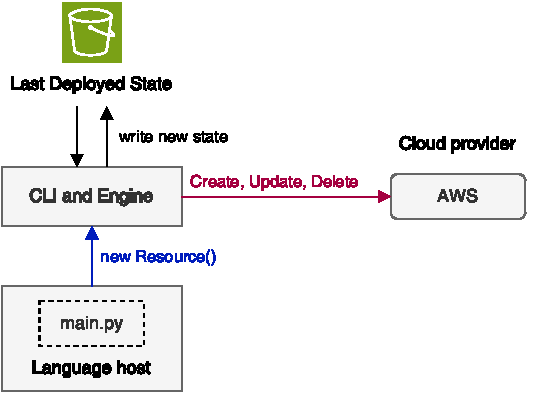
\includegraphics[width=.7\columnwidth]{implementation/pulumi_overview.pdf}
    \captionof{figure}{Overview of Pulumi's integration into the reference architecture}
    \label{fig:pulumi_overview}
    \endgroup
\end{center}
This \gls{cloud_infrastructure} part is implemented in a specific folder as follows :
\begin{center}
    \usemintedstyle{pastie}
    \begin{minted}
    [
    fontsize=\scriptsize
    ]{text}
    cloud-infrastructure
        ├── Pulumi.yaml
        ├── Pulumi.dev.yaml
        ├── Pulumi.prod.yaml
        ├── main.py
        ├── iam.py
        └── requirements.txt
    \end{minted}
\end{center}
The main configuration file for the Pulumi tool, \textit{Pulumi.yaml}, includes crucial information such as the name of the stack and the programming language used, in this case Python.

This implementation aims to facilitate the deployment of two distinct infrastructures, namely the development environment and the production environment. Therefore, two additional configuration files, \textit{Pulumi.dev.yaml} and \textit{Pulumi.prod.yaml}, are present to differentiate these two environments. \textit{Pulumi.dev.yaml} contains parameters such as the \gls{aws} development account ID and the deployment region, while \textit{Pulumi.prod.yaml} includes the same parameters with production-specific values. The identifiers of the \gls{aws} accounts must be different.

The Python files \textit{main.py} and \textit{iam.py} detail the description of the resources to be deployed. \textit{iam.py} focuses on IAM roles and policies, while \textit{main.py} mainly covers resources related to \acrshort{iot} and other resources.

Finally, the \textit{requirements.txt} file lists the Pulumi libraries to be installed, including the main Pulumi library, which is essential for all \acrshort{iac} projects.

In terms of the Pulumi libraries used, \gls{aws} Native, a new preview, uses the \gls{aws} \Gls{cloud} Control API to manage and provision \gls{aws} resources, generally aligning with the latest \gls{aws} features as they are released. The resources available in this library are based on those defined in the \gls{aws} CloudFormation registry. In addition, \gls{aws} Classic is another library that is used to fill in resources that are not yet available in \gls{aws} Native. This library uses the \gls{aws} SDK to manage and provision these resources.


\subsection{Embedded systems integration}
\subsubsection{\gls{aws} \acrshort{iot} Greengrass}
Integrating embedded systems with the \gls{aws} ecosystem is crucial to reaping the full benefits of \hyperref[subsec:cloudcomputing]{cloud computing}. To this end, \gls{aws} \acrshort{iot} Greengrass was chosen, a powerful solution that facilitates the execution of local processing on \acrshort{iot} devices, while enabling seamless interaction with \gls{aws} \gls{cloud} services. \gls{aws} defined this solution as follows :
\begin{quote}
    \textit{\gls{aws} \acrshort{iot} Greengrass is an open source \acrfull{iot} edge runtime and \gls{cloud} service that helps you build, deploy and manage \acrshort{iot} applications on your devices. You can use \gls{aws} \acrshort{iot} Greengrass to build software that enables your devices to act locally on the data that they generate, run predictions based on machine learning models, and filter and aggregate device data. \gls{aws} \acrshort{iot} Greengrass enables your devices to collect and analyze data closer to where that data is generated, react autonomously to local events, and communicate securely with other devices on the local network. Greengrass devices can also communicate securely with \gls{aws} \acrshort{iot} Core and export \acrshort{iot} data to the \gls{aws} Cloud. You can use \gls{aws} \acrshort{iot} Greengrass to build edge applications using pre-built software modules, called components, that can connect your edge devices to \gls{aws} services or third-party services. You can also use \gls{aws} \acrshort{iot} Greengrass to package and run your software using Lambda functions, Docker containers, native operating system processes, or custom runtimes of your choice. \cite{aws_iot_greengrass}}\\
\end{quote}
In this implementation, \gls{aws} \acrshort{iot} Greengrass Core software is deployed on embedded systems, acting as an intelligent hub that manages interactions with the \gls{aws} \gls{cloud}. It adapts perfectly to Linux \acrshort{os}. Greengrass components, encapsulating the necessary code, dependencies and resources, are then deployed automatically using mechanisms such as \gls{aws} \acrshort{iot} Greengrass Deployment.

A component must be installed. \textit{Greengrass nucleus} (aws.greengrass.Nucleus) is a mandatory component and the minimum requirement for running \gls{aws} \acrshort{iot} Greengrass Core software on a device. It is configurable to customize and update the \gls{aws} \acrshort{iot} Greengrass Core software \acrlong{ota}.

\subsubsection{Communication}
In this project, components running on an embedded system use the \gls{aws} \acrshort{iot} Greengrass Core \acrfull{ipc} library, available in the \gls{aws} \acrshort{iot} Device SDK, to exchange data with the \gls{aws} \acrshort{iot} Greengrass nucleus and other Greengrass components. The \acrshort{ipc} interface supports the \acrlong{mqtt} communication protocol. \acrshort{mqtt} offers lightweight, asynchronous communication.

Publish/subscribe messaging allows messages to be sent and received in topics. Components can publish messages in topics to communicate with other components, and those who have subscribed to the topic can act on messages received. In this case, the communication is local to the \acrshort{iot} device.

The \acrshort{ipc} interface also facilitates the sending and receiving of \acrshort{mqtt} messages between \gls{aws} \acrshort{iot} Greengrass and \gls{aws} \acrshort{iot} Core. Components can publish messages to \gls{aws} \acrshort{iot} Core and subscribe to topics to react to \acrshort{mqtt} messages from other sources.

\subsubsection{\acrshort{ota} update}
All devices with \gls{aws} \acrshort{iot} Greengrass Core software can obtain \acrshort{ota} updates via \acrshort{mqtt}.

\textbf{\gls{aws} \acrshort{iot} Greengrass Core software update}\\
This functionality is built into the \gls{aws} \acrshort{iot}Greengrass Core software. It is made possible by the \textit{Greengrass nucleus} component and other optional components. The following information is taken from the \gls{aws} documentation \cite{ota_aws_iot}.

A few prerequisites must be met before an update can be carried out. Firstly, the Greengrass device must be connected to the \gls{cloud} \gls{aws} in order to receive the deployment. It must be properly configured with certificates and authentication keys to interact with both the \gls{aws} \acrshort{iot} Core and \gls{aws} \acrshort{iot} Greengrass. Finally, the \gls{aws} \acrshort{iot} Greengrass Core software must be configured and run as a system service.

There are a few things to bear in mind when upgrading. The Greengrass nucleus stops. This stops all the other components present. When the nucleus component is shut down, the device's connection to \gls{aws} is lost.

The following table summarises the behaviour of Greengrass updates :

\begin{tabularx}{1\textwidth} { 
    | >{\raggedright\arraybackslash}X 
    | >{\raggedright\arraybackslash}X 
    | >{\raggedright\arraybackslash}X | }
    \hline
    \rowcolor{lightgray}
    Action              & Deployment configuration  & Nucleus update behavior \\ \hline
    \multirow{2}{\linewidth}{Add new devices to a thing group targeted by an existing deployment without revising the deployment.}
    & The deployment does not directly include Greengrass nucleus.
    
    The deployment directly includes at least one \gls{aws}-provided component, or includes a custom component that depends on an \gls{aws}-provided component or on the Greengrass nucleus.
    & On new devices, installs the latest patch version of nucleus that meets all component dependency requirements.

    On existing devices, does not update the installed version of the nucleus. \\ \cline{2-3}
    & The deployment directly includes a specific version of the Greengrass nucleus.
    & On new devices, installs the specified nucleus version.

    On existing devices, does not update the installed version of the nucleus. \\ \hline
    \multirow{2}{\linewidth}{Create a new deployment or revise an existing deployment.}
    & The deployment does not directly include Greengrass nucleus.

    The deployment directly includes at least one \gls{aws}-provided component, or includes a custom component that depends on an \gls{aws}-provided component or on the Greengrass nucleus.
    & On all targeted devices, installs the latest patch version of the nucleus that meets all component dependency requirements, including on any new devices that you add to the targeted thing group. \\ \cline{2-3} 
    & The deployment directly includes a specific version of the Greengrass nucleus.
    & On all targeted devices, installs the specified nucleus version, including any new devices that you add to the targeted thing group. \\ \hline
\end{tabularx}

In this reference architecture, the version of \textit{Greengrass nucleus} is not specified. However, there is one component provided by \gls{aws} (\textit{aws.greengrass.Cli}) and custom components which depend on several components provided by \gls{aws}.

\textbf{Greengrass components update}\\
For custom or public \gls{aws} components, the \gls{aws} \acrshort{iot} Greengrass Deployment service enables OTA updates.

The prerequisites for an update are the same as for the software update. When an update is deployed, only components with a new version are updated. These components will then be stopped and restarted automatically after being updated. If a deployment error occurs, a rollback is performed and the components resume their course with the old version.

The following table explains two main actions:

\begin{tabularx}{1\textwidth} { 
    | >{\raggedright\arraybackslash}X
    | >{\raggedright\arraybackslash}X | }
    \hline
    \rowcolor{lightgray}
    Action              & Components behaviour \\ \hline
    Add new devices to a group of devices targeted by an existing deployment without modifying the deployment.
    & All the components and dependencies present in the deployment are automatically deployed with their latest version on the new devices.
    
    On existing devices, nothing happens.\\
    \hline
    Create a new version of one or more Greengrass components.
    & Only components with a new version will be deployed on all devices in the group of devices targeted for deployment. \\
    \hline
\end{tabularx}

\subsubsection{Fleet \gls{provisioning}}
With \gls{aws} \acrshort{iot} fleet \gls{provisioning}, it is possible to securely set up \gls{aws} \acrshort{iot} to generate and distribute X.509 device certificates and private keys to each device when they first connect to \gls{aws} \acrshort{iot} \cite{aws_iot_greengrass_fleet}. These client certificates, signed by the Amazon Root Certificate Authority, are provided by \gls{aws} \acrshort{iot}. It is very flexible to define specific device groups, device types and permissions for Greengrass Core devices to be provisioned using fleet \gls{provisioning}. A \gls{provisioning} template is used to describe the \gls{provisioning} process for each device, detailing the device, policy and certificate resources to be created during \gls{provisioning}. This template is created from Pulumi.

\gls{aws} \acrshort{iot} Greengrass offers a dedicated \gls{aws} \acrshort{iot} fleet \gls{provisioning} plugin (\textit{aws.greengrass .FleetProvisioningByClaim}), which facilitates the installation of \gls{aws} \acrshort{iot} Greengrass Core software using the resources created by \gls{aws} \acrshort{iot} fleet \gls{provisioning}. This plugin uses claim-based \gls{provisioning}, where devices use a \gls{provisioning} claim certificate and private key to obtain a unique X.509 device certificate, along with a private key, enabling regular operations. The claim certificate and private key are integrated as soon as the Linux \acrshort{os} image is created, enabling devices to be activated later when they are connected. The same claim certificate and private key can be used for multiple devices.

To deploy \gls{aws} \acrshort{iot} Greengrass Core software with \gls{aws} \acrshort{iot} fleet provisioning, configuration of resources in the \gls{aws} account is required. These resources include a provisioning template, a claim certificate and a token exchange IAM role. Once these elements have been created from Pulumi, apart from the certificate from the \gls{aws} \acrshort{cli}, they can be reused to provision several embedded systems within the same fleet. The token exchange IAM role authorises calls to \gls{aws} services from the \acrshort{iot} device.

In this architecture, devices are registered by their serial number to ensure that each one has a unique name.

\subsubsection{\acrshort{os} image}
To enable the devices to be provisioned to integrate automatically on their first boot, a Linux \acrshort{os} image is created specifically for this purpose. The base image used for this architecture is \textit{Raspberry Pi \acrshort{os} Lite} based on the Debian distribution. A directory dedicated to the creation of the image is present as follows:
\begin{center}
    \usemintedstyle{pastie}
    \begin{minted}
    [
    fontsize=\scriptsize
    ]{text}
    os-image
        ├── raspios-lite.json
        ├── set_os.sh
        ├── provision.sh
        └── config.yaml
    \end{minted}
\end{center}
Image creation is managed by Packer \cite{packer}, an open source tool for automating image creation. Packer follows a process defined in a configuration file \acrshort{json} (\textit{raspios-lite.json}).

It works as follows :
\begin{enumerate}
    \item \textbf{Packer configuration} (raspios-lite.json) : The Packer configuration file describes all the steps required to create the image. It specifies the constructors (in this case, the Arm constructor), the actions to be performed, the base image sources and other parameters.
    \item \textbf{Running Packer} : In this project, Packer runs in a Docker environment. When the container is launched, the tool starts the build process following the specified configuration.
    \item \textbf{Packer builder ARM plugin} : A plugin \cite{packer_plugin} to the Packer tool is used to build images specific to the Arm architecture. It uses the Arm build model to create a custom image based on the specification.
    \item \textbf{Actions} : The actions in the configuration file are carried out to configure the image. This may involve installing software, configuring system parameters, etc. In this case, some system parameters are configured using the \textit{set\_os.sh} script. The \gls{provisioning} script \textit{provision.sh} used to install the necessary software is saved in the image and configured to run the first time the operating system is booted. Finally, the claim certificate and its private key are saved in the image.
    \item \textbf{Build complete} : Once all the build and configuration steps have been successfully completed, Packer creates a custom image in the specified format (.img in this case).
\end{enumerate}

The \gls{provisioning} file \textit{provision.sh} is a bash script. When it first runs on a device, it first retrieves the device's serial number, so that the device is registered in \gls{aws} \acrshort{iot} under that name. The script then installs the Docker Engine software, paving the way for future deployment of Greengrass components in containers. After this step, \gls{aws} \acrshort{iot} Greengrass Core is installed with the plugin specially dedicated to fleet \gls{provisioning}. Finally, the \gls{provisioning} command is executed using the \textit{config.yaml} configuration file, which contains various parameters such as the device serial number, as well as the paths to locate the claim certificate and private key.

\subsection{Security}
At \gls{aws}, security is a top priority \cite{aws_iot_greengrass_security}. Security is a shared responsibility between \gls{aws} and the developer :
\begin{itemize}
    \item \textbf{Security of the \gls{cloud}} : \gls{aws} is responsible for protecting the infrastructure that runs \gls{aws} services in the \gls{aws} \gls{cloud}.
    \item \textbf{Security in the \gls{cloud}} : The developer's responsibility is determined by the \gls{aws} service that he uses.
\end{itemize}
When using \gls{aws} \acrshort{iot} Greengrass, the developer is also responsible for securing these devices, the connection to the local network and the private keys.

\subsubsection{Authentication}
Greengrass devices use X.509 certificates for authentication. X.509 certificates are digital certificates that adopt the X.509 public key infrastructure standard to bind a public key to the identity specified in the certificate. These X.509 certificates are issued by a trusted entity known as a \acrfull{ca}. The \acrshort{ca} holds one or more specific certificates, called \acrshort{ca} certificates, which it uses to issue X.509 certificates. Only this \acrshort{ca} has the privilege of accessing the certificates. In this process, the authority is Amazon Root \acrlong{ca}. When \gls{provisioning} a device, the fleet \gls{provisioning} plugin requests a unique client certificate from this authority. \cite{aws_iot_greengrass_security}

Only devices authorised to be provisioned will receive a certificate. In this implementation, a list allowing the serial numbers of authorised devices to be inserted has been created in a dedicated file (\textit{allowlist.txt}). When the \gls{provisioning} plugin attempts to provision a device, it will first trigger a Lambda function which will check the list to see if the device is authorised. If so, it will receive its unique certificate. If not, it will not receive it and will not be provisioned.

Greengrass devices store certificates in the default Greengrass root folder (\textit{/v2/greengrass/}).

\subsubsection{Authorization}
Greengrass devices rely on \gls{aws} \acrshort{iot} policies for authorization. These \gls{aws} \acrshort{iot} policies determine the scope of operations permitted for \gls{aws} \acrshort{iot} devices. They specify, in detail, permissions or denials of access to \gls{aws} \acrshort{iot} Core and \gls{aws} \acrshort{iot} Greengrass data plane operations, including actions such as publishing \acrshort{mqtt} messages. In this architecture, an \gls{aws} \acrshort{iot} policy is created directly from Pulumi. \cite{aws_iot_greengrass_security}

\subsubsection{Data protection}
Greengrass devices frequently collect data for transmission to \gls{aws} services for further processing. \gls{aws} \acrshort{iot} Greengrass uses encryption to protect data in transit (via the internet or local network) and at rest (stored in the \gls{aws} \gls{cloud}). \cite{aws_iot_greengrass_security}

\gls{aws} \acrshort{iot} Greengrass offers two distinct modes of communication for data in transit :
\begin{itemize}
    \item \textbf{Data in transit over the internet} : Communication over the internet between a device and \gls{aws} \acrshort{iot} is encrypted using the \acrfull{tls} protocol. \acrshort{tls} is a security protocol that guarantees the confidentiality and integrity of data when it is exchanged over a network. All data sent to the \gls{aws} \gls{cloud} therefore uses the \acrshort{mqtt} protocol based on \acrshort{tls}.
    \item \textbf{Data on the device} : Communication between components on the Greengrass device is not encrypted, as the data does not leave the device.
\end{itemize}

When it comes to data at rest, \gls{aws} \acrshort{iot} Greengrass adopts different approaches :
\begin{itemize}
    \item \textbf{Data at rest in the \gls{aws} \gls{cloud}} : Customer data stored in the \gls{aws} \gls{cloud} is encrypted by the \gls{aws} \acrshort{iot} Greengrass service using \gls{aws} KMS keys under its management.
    \item \textbf{Data at rest on the Greengrass device} : Data at rest on the device is protected by Unix file permissions and full disk encryption (if enabled, not enabled in this implementation). The user is responsible for securing the file system and the device.
\end{itemize}

% -----------------------------------------------------------------------------
\section{\texorpdfstring{\acrshort{ci}/\acrshort{cd}}{} pipeline}
A \acrshort{ci}/\acrshort{cd} process derived from the \acrshort{devops} methodology has been put in place. It automates several workflows by integrating all the tools and software already described. The entire reference architecture has been developed in a public GitHub repository \cite{aws_iot_reference_architecture}.

% -- Your text goes here --
\subsection{GitHub Actions}
GitHub Actions is the \acrfull{ci} and \acrfull{cd} service integrated directly into the GitHub platform and used in this project. It automates various aspects of the software development lifecycle, from building code to deploying it.

GitHub Actions works like this :
\begin{enumerate}
    \item \textbf{Definition of workflows} : These describe the specific steps to be carried out during particular events, such as code validations, new version releases, etc. Several workflows can be run sequentially or in parallel.
    \item \textbf{Triggering workflows} : These are triggered automatically in response to specific events defined by the developers. For example, a workflow can be triggered every time a new branch is created.
    \item \textbf{Execution of steps} : Each workflow is made up of steps (jobs) that are executed sequentially or in parallel. These steps can include predefined actions, custom scripts, tests, deployments, etc.
    \item \textbf{Runtime environments} : GitHub Actions provides runtime environments managed by GitHub. In this context, the Ubuntu-based Linux environment is used.
    \item \textbf{Notifications and reports} : The results of each stage of the workflow are recorded and presented in the GitHub interface. Developers can receive notifications of successful or unsuccessful execution of the workflow.
    \item \textbf{Integration with other services} : GitHub Actions can be integrated with other services and tools, such as cloud deployment services, notification services, secret management tools, etc.
    \item \textbf{Actions ecosystem} : GitHub Actions offers a rich ecosystem of pre-built actions that developers can use in their workflows. These actions are reusable units of functionality (tests, deployments, notifications, etc.).
\end{enumerate}

All workflows are implemented in a specific folder as follows :
\begin{center}
    \usemintedstyle{pastie}
    \begin{minted}
    [
    fontsize=\scriptsize
    ]{text}
    .github/workflows
        ├── deploy-infra.yml
        ├── setup-provisioning.yml
        ├── build-image.yml
        ├── test-apps.yml
        ├── build-apps.yml
        ├── deploy-apps.yml
        └── destroy-infra.yml
    \end{minted}
\end{center}

\subsection{Access to \gls{aws} resources}
GitHub Actions integrates seamlessly with the \gls{aws} \gls{cloud}. It uses the \acrfull{oidc} credentials protocol to access resources when deploying or updating the \gls{cloud_infrastructure}. \acrshort{oidc} allows workflows to interact with \gls{aws} \gls{cloud} service provider resources without having to permanently store credentials as GitHub secrets. Before deploying the infrastructure, the \gls{aws} account configuration is adjusted to recognise the GitHub \acrshort{oidc} as a trusted federated identity. In addition, this identification is based on IAM roles. This limits the possible actions on resources to the minimum required. Everything must be configured before the \acrshort{ci}/\acrshort{cd} process is launched.

To enable this connection to be used, \gls{aws} provides a pre-built action which is integrated into the flows (\textit{aws-actions/configure-aws-credentials}).

\subsection{Infrastructure deployment}
This initial flow is triggered each time a new modification is pushed into Git. Before deploying the \gls{cloud_infrastructure}, the decision was taken to generate a claim certificate and store it in a dedicated S3 bucket. This operation is carried out only once, ensuring that the same claim certificate is always preserved, even if the infrastructure is destroyed and redeployed at a later date. This ensures that devices ready to be provisioned can always do so using the same claim certificate.

A second S3 bucket is specifically created to record the state of the infrastructure. Pulumi connects to it, orchestrating the deployment of the configured infrastructure, whether for the development or production environment.

Successful completion of this first stage simultaneously triggers two other processes: provisioning configuration and testing of the developed applications. If deployment fails, the entire \acrshort{ci}/\acrshort{cd} process is interrupted.
\begin{center}
    \begingroup
    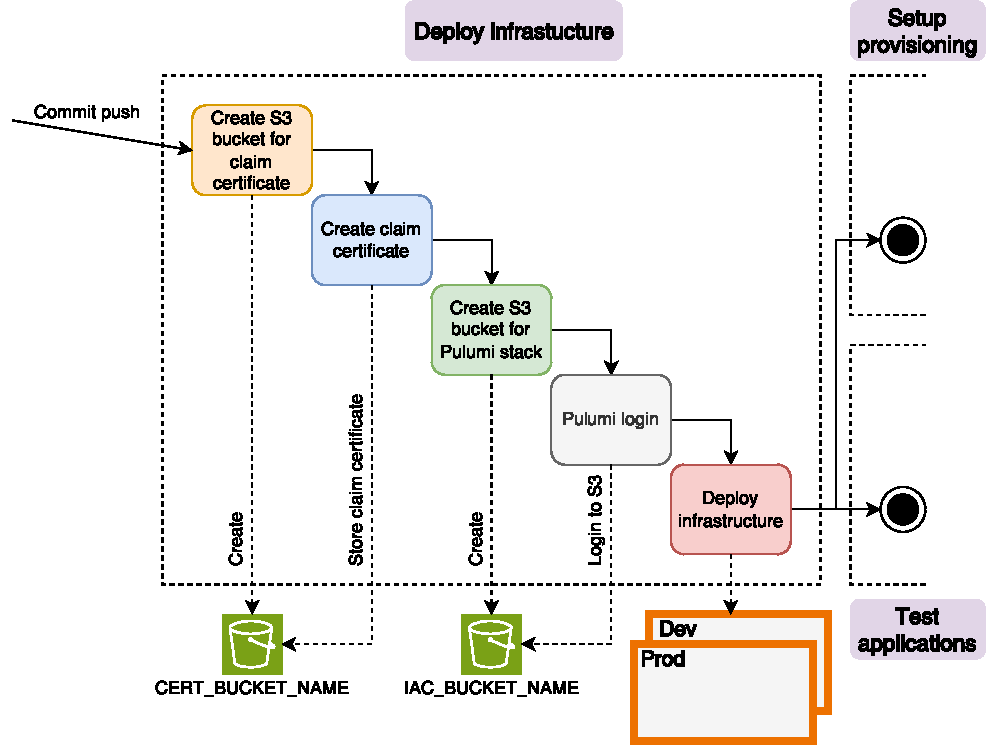
\includegraphics[width=1\columnwidth]{implementation/deploy_infra.pdf}
    \captionof{figure}{Infrastructure deployment workflow}
    \label{fig:deploy_infra}
    \endgroup
\end{center}

\subsection{\Gls{provisioning} setup}
This flow manages the preparation of configuration files for provisioning embedded systems, as well as checking devices that have already been provisioned. Two tasks are performed simultaneously. The first checks the serial numbers of devices in a dedicated list. If previously provisioned devices are no longer in the list, they are removed from the \gls{aws} \gls{cloud}. Authorised devices are reassigned to the new infrastructure and their unique certificate is reassociated with the \gls{aws} \acrshort{iot} policy for actions in the \gls{cloud}.

The second task, related to configuration, retrieves the \acrshort{iot} endpoints for future communications between the devices and \gls{aws} \acrshort{iot}. Next, the parameters are saved in a configuration file required for provisioning. This file is stored, along with the list of authorised devices, in the same S3 bucket as the claim certificate.

Only if this flow is successful will the creation of the Linux image begin.
\begin{center}
    \begingroup
    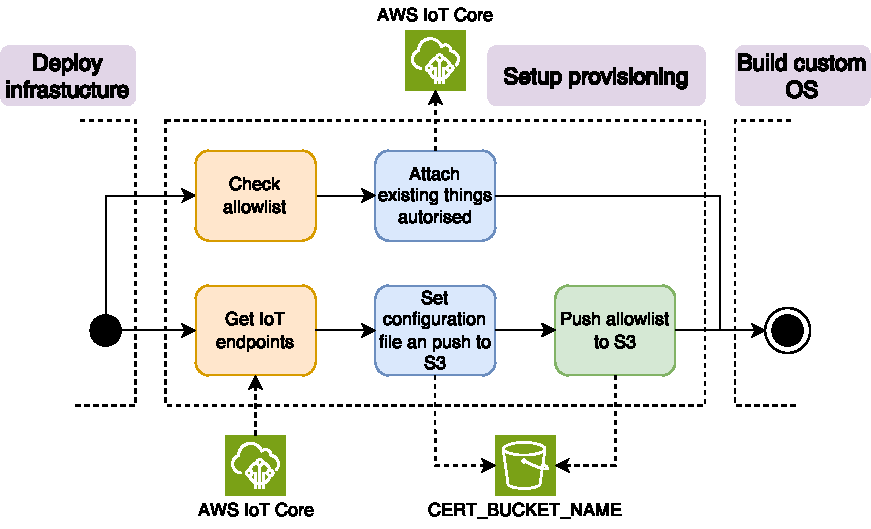
\includegraphics[width=.9\columnwidth]{implementation/setup_provisioning.pdf}
    \captionof{figure}{\Gls{provisioning} setup workfow}
    \label{fig:setup_provisioning}
    \endgroup
\end{center}

\subsection{\acrshort{os} image building}
This process begins by retrieving the configuration file and the claim certificate, along with its associated private key, which have previously been saved in the S3 compartment. The image is then created using the Packer tool and its plugin. The image is created in a Docker container preconfigured with the necessary environment. Once the image has been generated, it is saved in its corresponding S3 compartment.
\begin{center}
    \begingroup
    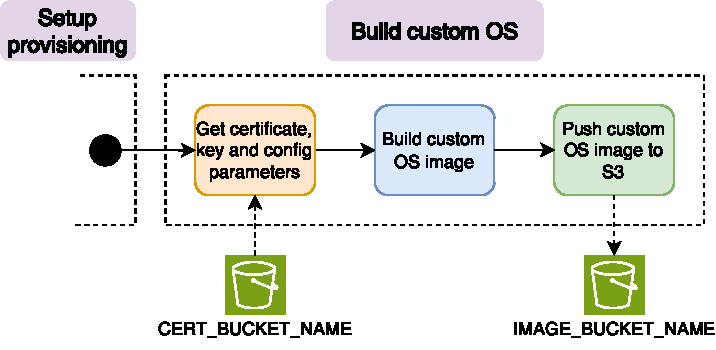
\includegraphics[width=.7\columnwidth]{implementation/build_os.pdf}
    \captionof{figure}{\acrshort{os} image building workflow}
    \label{fig:build_os}
    \endgroup
\end{center}

\subsection{Applications testing}
Simultaneously with the two previous workflows, this stage aims to test all the applications developed. It runs three tests concurrently. The first tests the linting of each application, helping to improve the quality of the code. The second performs static security tests for each application. Finally, unit tests are carried out using test code developed in parallel with the applications. The tools used in this task will depend on the programming language used.

If all the tests have been passed, the applications can be built.
\begin{center}
    \begingroup
    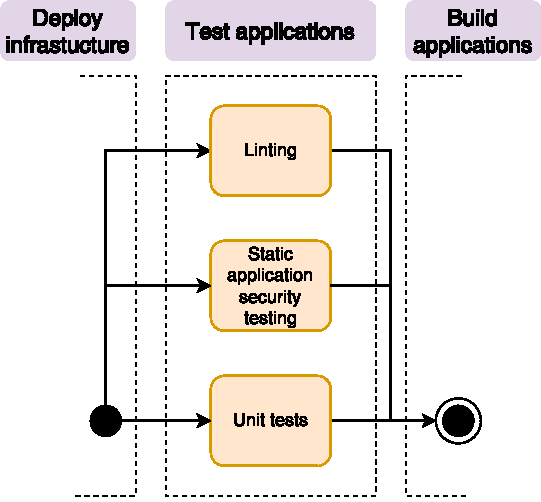
\includegraphics[width=.6\columnwidth]{implementation/test_apps.pdf}
    \captionof{figure}{Applications testing workflow}
    \label{fig:test_apps}
    \endgroup
\end{center}

\subsection{Applications building}
This process is divided into two stages. The first involves containerising applications using Docker, with this operation applied only to new applications or those that have undergone modifications. The resulting images are then stored in the dedicated Amazon \acrshort{ecr} service.

The second part of the process focuses on creating a Greengrass component for each application. When a component is updated, a new version is created. However, only applications that have undergone modifications will see a new version of their component generated. It is also possible for a component's parameters to change, causing it to be updated. Each time a new version of a component is released, it is published in \gls{aws} \acrshort{iot} Greengrass, orchestrated by the \gls{aws} Greengrass Development Kit (GDK).

Once this workflow has been successfully completed, the Greengrass components are deployed.
\begin{center}
    \begingroup
    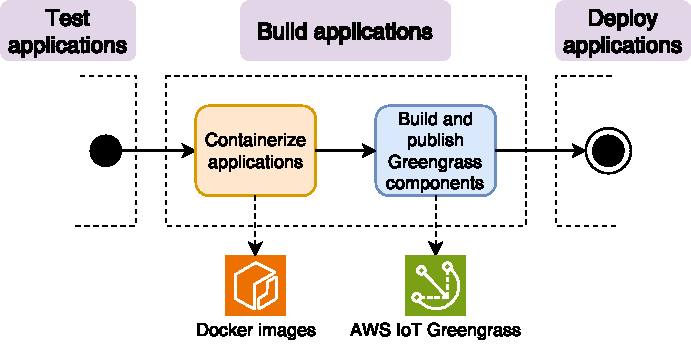
\includegraphics[width=.7\columnwidth]{implementation/build_apps.pdf}
    \captionof{figure}{Applications building workflow}
    \label{fig:build_apps}
    \endgroup
\end{center}

\subsection{Applications deployment}
This workflow supports the deployment of Greengrass components on a group of devices. It does this using the \gls{aws} \acrshort{cli}. It doesn't matter whether the components have been updated or not, deployment takes place either way. \gls{aws} \acrshort{iot} Greengrass Deployment is smart enough to see if a new version of a component has been released. If this is the case, only the component with the new version will be deployed in the device group.
\begin{center}
    \begingroup
    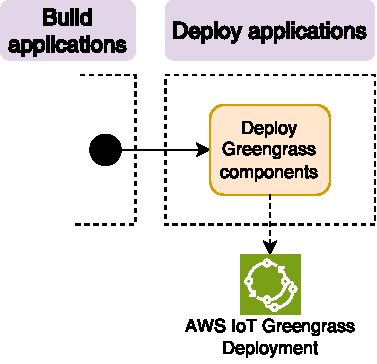
\includegraphics[width=.4\columnwidth]{implementation/deploy_apps.pdf}
    \captionof{figure}{Applications deployment workflow}
    \label{fig:deploy_apps}
    \endgroup
\end{center}

\subsection{Infrastructure destruction}
This last workflow is optional and has the task of dismantling the \gls{aws} \gls{cloud_infrastructure}. To enable Pulumi to delete the S3 bucket containing the \acrshort{os} image, it must first be emptied. The \acrshort{os} image is then deleted. The bucket containing the configuration file and the list of authorised devices is emptied, with the exception of the claim certificate and its private key. Embedded systems integrated into the \gls{aws} \gls{cloud} retain their unique certificate in \gls{aws}, but lose their \gls{aws} \acrshort{iot} policy, dissociating them from any action. Finally, Pulumi connects to the S3 bucket containing the stack to completely remove the infrastructure. Once all the operations have been completed, the S3 bucket containing the stack is also deleted.
\begin{center}
    \begingroup
    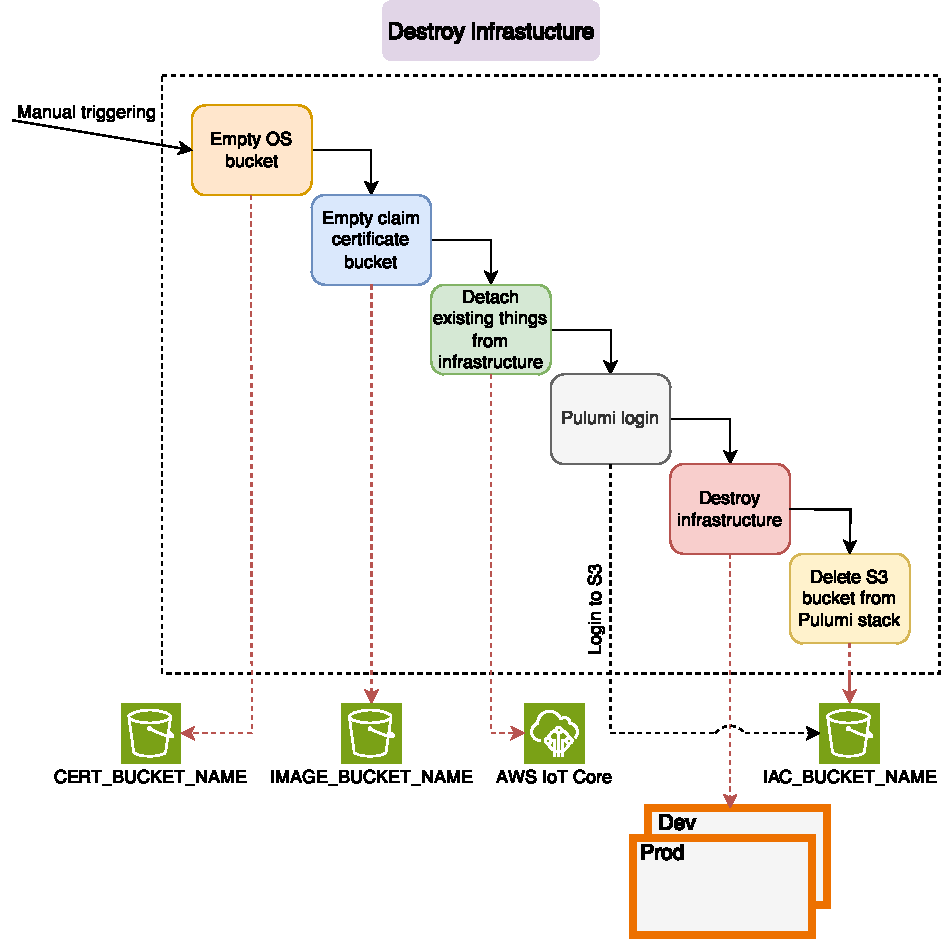
\includegraphics[width=1\columnwidth]{implementation/destroy_infra.pdf}
    \captionof{figure}{Infrastructure destruction workflow}
    \label{fig:destroy_infra}
    \endgroup
\end{center}

% ------------------------------------------------------------------------------
\section{Applications}

% -- Your text goes here --
\subsection{Greengrass components}
Greengrass components are software modules that are deployed on devices containing the \gls{aws} \acrshort{iot} Greengrass Core program. Components can be applications, runtime installers, libraries, or any code that is executable on a device. Components may depend on other components. For example, one component installs Python and other components depend on it to run Python applications. When components are deployed on a fleet of devices, \gls{aws} \acrshort{iot} Greengrass deploys only the software modules that the devices need. \cite{aws_iot_greengrass_components}

Here are some key points about Greengrass components :
\begin{itemize}
    \item \textbf{Greengrass component definition} : A component can be defined as a combination of code (for example, a Python application), software dependencies and system resources. These may include libraries, configuration files, executables, etc.
    \item \textbf{Component management} : \gls{aws} \acrshort{iot} Greengrass enables centralised management of components. Components can be created, published and managed in \gls{aws} \acrshort{iot} Greengrass and deployed to groups of Greengrass devices.
    \item \textbf{Types of components} : Two types of component are used
    \begin{itemize}
        \item Nucleus (aws.greengrass.nucleus): The Greengrass nucleus is the mandatory installed component that provides the minimum functionality for the operation of the \gls{aws} \acrshort{iot} Greengrass Core software.
        \item Generic (aws.greengrass.generic): The Greengrass nucleus executes lifecycle scripts for a generic component. This type is the default for custom components.
    \end{itemize}
    \item \textbf{Deployment} : Components are deployed on groups of Greengrass devices to run device-level applications. Deployments are orchestrated and managed from the \gls{aws} \acrshort{iot} Greengrass Deployment service.
    \item \textbf{Versioning} : Components can be versioned, enabling different versions of the software to be managed and updates to be rolled out in a controlled manner.
\end{itemize}

In this project, a component is defined in a folder as follows :
\begin{center}
    \usemintedstyle{pastie}
    \begin{minted}
    [
    fontsize=\scriptsize
    ]{text}
    component_1
        ├── gdk-config.json
        └── recipe.yaml
    \end{minted}
\end{center}
The \textit{gdk-config.json} file is specific to the \gls{aws} GDK tool, used to generate and publish a component to \gls{aws} \acrshort{iot} Greengrass. It only includes parameters such as the component name, for example.

The \textit{recipe.yaml} file describes the component, its required dependencies, its lifecycle and the location of the executable. An example of this file is shown below.
\begin{center}
    \usemintedstyle{pastie}
    \begin{minted}
    [
    fontsize=\scriptsize
    ]{yaml}
    RecipeFormatVersion: "2020-01-25"
    ComponentName: COMPONENT_NAME
    ComponentVersion: COMPONENT_VERSION
    ComponentDescription: COMPONENT_DESCRIPTION
    ComponentPublisher: AUTHOR
    ComponentConfiguration:
        DefaultConfiguration:
            var1: 1
            var2: "frequency"
            accessControl:
                aws.greengrass.ipc.mqttproxy:
                    com.app:mqttproxy:1:
                        policyDescription: "Allows access to subscribe to input topics from AWS IoT."
                        operations:
                            - "aws.greengrass#SubscribeToIoTCore"
                        resources:
                            - "topic1"
                    com.app:mqttproxy:2:
                        policyDescription: "Allows access to publish to output topics to AWS IoT."
                        operations:
                            - "aws.greengrass#PublishToIoTCore"
                        resources:
                            - "topic2"
    ComponentDependencies:
        aws.greengrass.DockerApplicationManager
    Manifests:
    - Platform:
        os: linux
        architecture: aarch64
      Lifecycle:
        run: 
            RequiresPrivilege: true
            Script: docker run DOCKER_IMAGE@DIGEST
      Artifacts:
        - URI: "docker:AWS_ACCOUNT_ID.dkr.ecr.AWS_REGION.amazonaws.com/DOCKER_IMAGE"
    \end{minted}
\end{center}
Starting at the top of the example, information about the component is presented. Next, the configuration (\textit{ComponentConfiguration}) is detailed, allowing the creation of variables and the configuration of access controls (\textit{accessControl}). The latter is used to define authorised operations, typically using the \acrshort{mqtt} protocol, such as the topics to which the component can publish or subscribe. Next, the dependent components are specified (\textit{ComponentDependencies}). Finally, the lifecycle (\textit{Lifecycle}) is detailed, along with the specification of the environment platform. In this example, a Docker application is launched and its image has been retrieved from the Amazon \acrshort{ecr} service via its URI.

\subsection{Containerization}
\label{sec:containerization}

The Python applications developed in this project are run in Docker containers. The creation of the application image requires the use of a Dockerfile. This specifies the architecture of the embedded system on which the container is to run, as well as the base image used. Finally, the Dockerfile copies the directory containing the application into its environment, then simply executes a bash script. This bash script installs the necessary Python libraries and launches the Python application.
\begin{center}
    \usemintedstyle{pastie}
    \begin{minted}
    [
    fontsize=\scriptsize
    ]{text}
    docker_app_1
        ├── app_1
        ├   ├── start.sh
        ├   ├── requirements.txt
        ├   └── main.py
        └── Dockerfile
    \end{minted}
\end{center}

\subsection{Certificate rotator application}
This application, which is essential to ensure that \acrshort{iot} devices work properly, has been implemented in Python. Figure \ref{fig:class_diagram_certificate_rotator_app} illustrates the associated class diagram.
\begin{center}
    \begingroup
    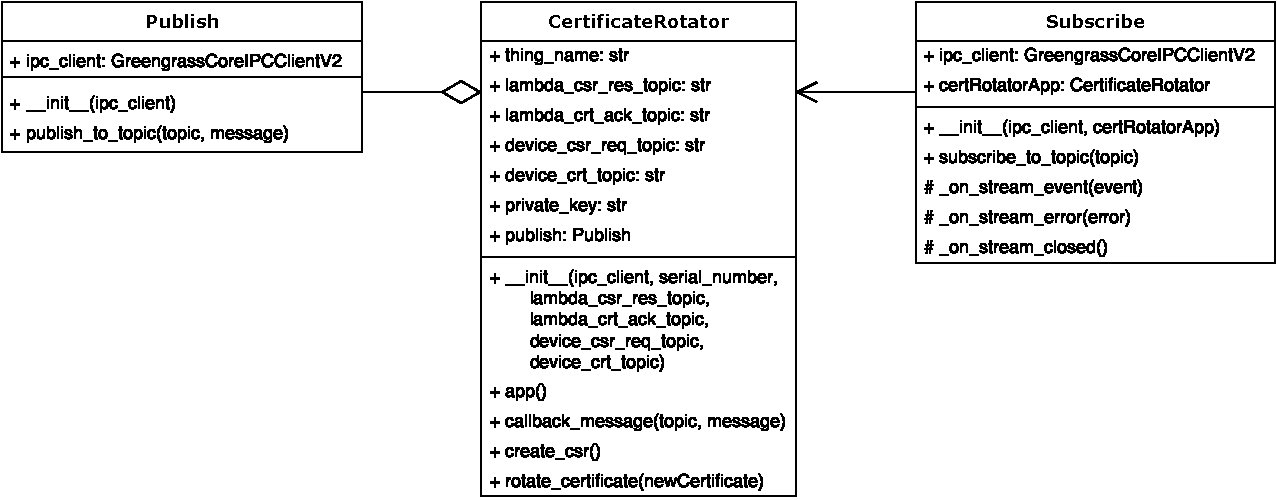
\includegraphics[width=1\columnwidth]{implementation/class_diagram_certificate_rotator_app.pdf}
    \captionof{figure}{Certificate rotation application class diagram}
    \label{fig:class_diagram_certificate_rotator_app}
    \endgroup
\end{center}
Below is a description of the various classes :
\begin{itemize}
    \item \textit{CertificateRotator} : Main class that includes the program's main loop. It generates \acrshort{csr} and private keys. It also changes the old certificates to the new ones received.
    \item \textit{Publish} : Class that publishes \acrshort{mqtt} messages to \gls{aws} \acrshort{iot}.
    \item \textit{Subscribe} : Class that receives \acrshort{mqtt} messages from \gls{aws} \acrshort{iot}.
\end{itemize}
A sequence diagram illustrating how the application works is available in figure \ref{fig:sequence_diagram_certificate_rotation_app}.
\begin{center}
    \begingroup
    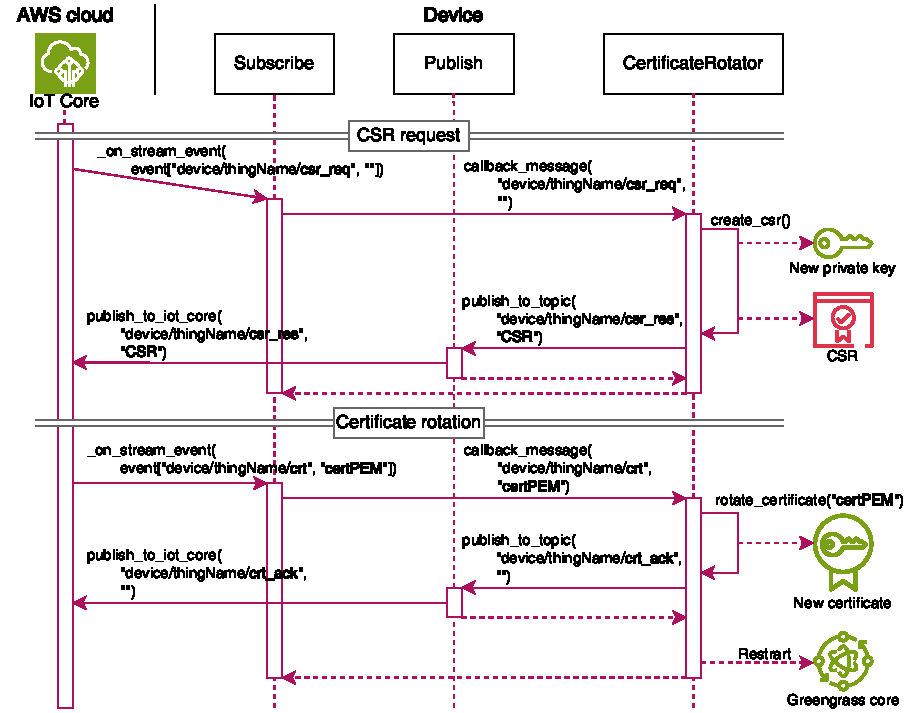
\includegraphics[width=.9\columnwidth]{implementation/sequence_diagram_certificate_rotation_app.pdf}
    \captionof{figure}{Certificate rotation application sequence diagram}
    \label{fig:sequence_diagram_certificate_rotation_app}
    \endgroup
\end{center}
The sequence diagram \ref{fig:sequence_diagram_certificate_rotation_app} highlights the two main actions of the application : the \acrfull{csr} and the certificate replacement. When the \acrshort{mqtt} broker integrated into \gls{aws} \acrshort{iot} Core transmits a message relating to the creation of the \acrshort{csr}, the corresponding method is triggered. This method then sends the \acrshort{csr} to \gls{aws} \acrshort{iot} Core, which responds by providing a new certificate, thus initiating the rotation process.

Another sequence diagram is shown in Figure \ref{fig:sequence_diagram_certificate_rotation}, detailing the process of integrating the application into the \acrshort{iot} device in collaboration with \gls{aws} services.
\begin{center}
    \begingroup
    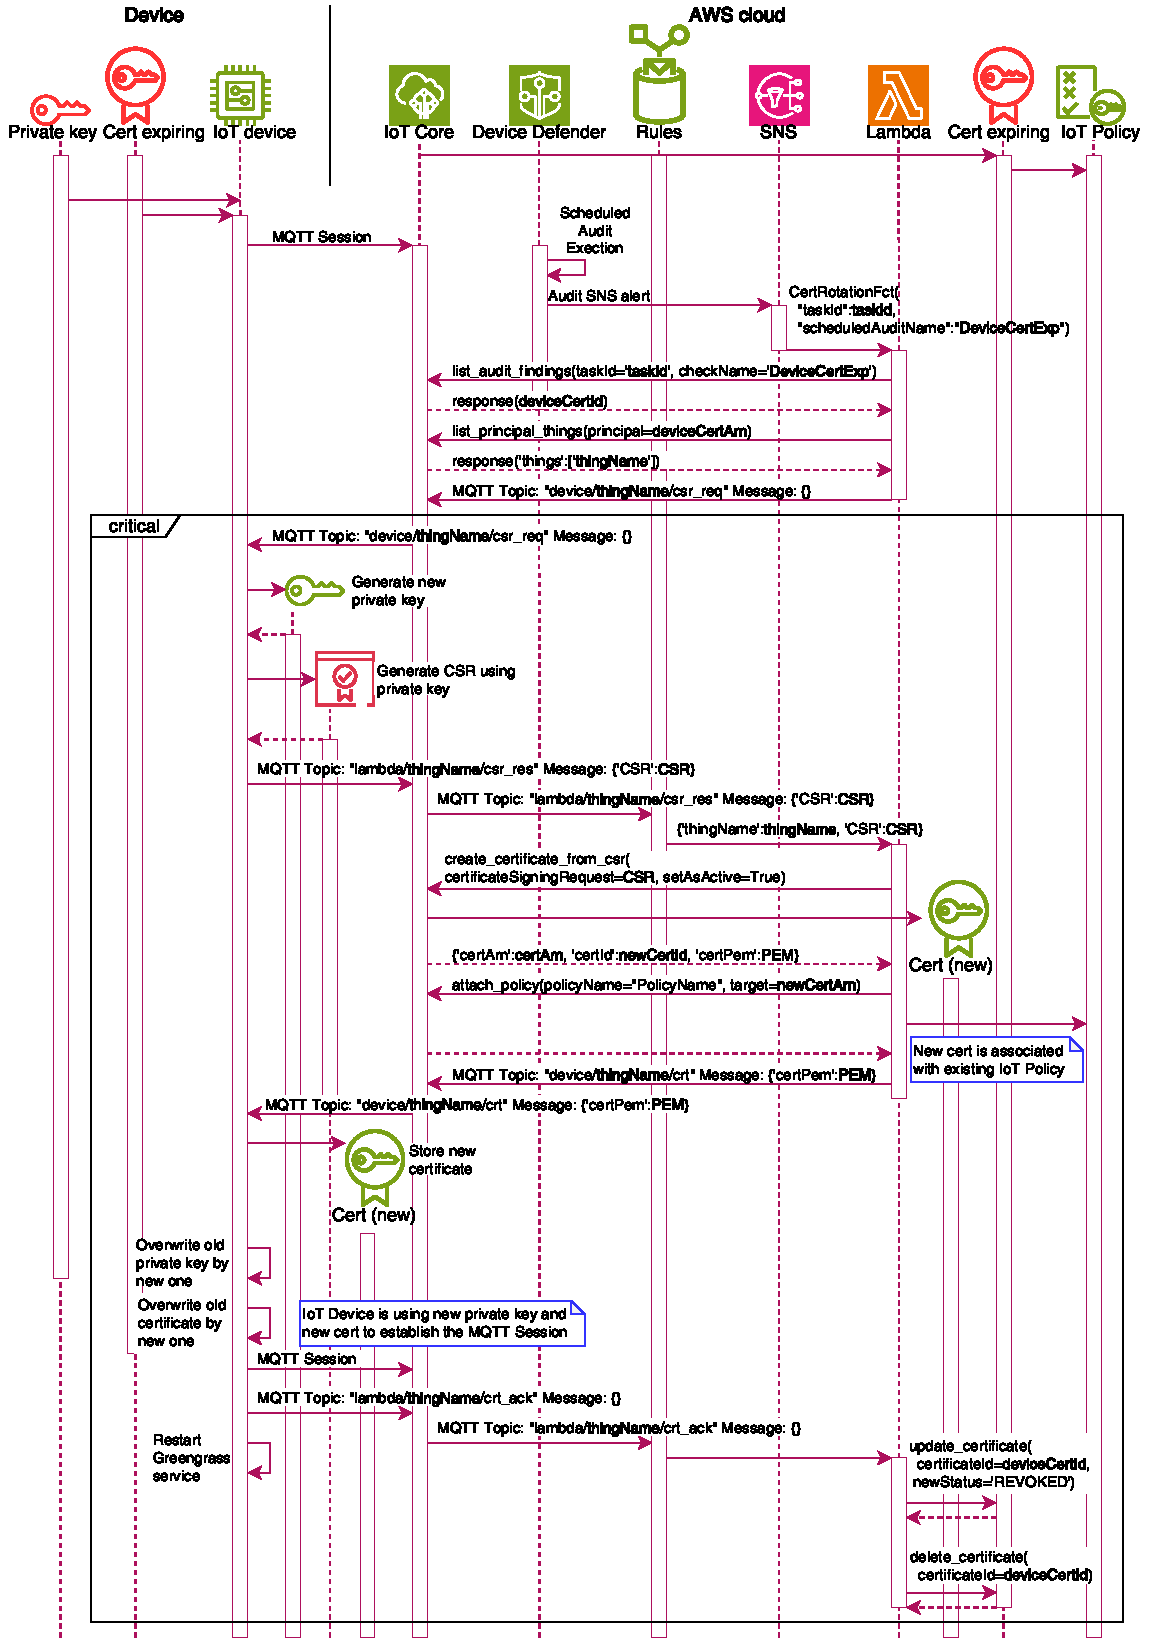
\includegraphics[width=1\columnwidth]{implementation/sequence_diagram_certificate_rotation.pdf}
    \captionof{figure}{Certificate rotation sequence diagram with \gls{aws} services \cite{aws_iot_certificate_rotator}}
    \label{fig:sequence_diagram_certificate_rotation}
    \endgroup
\end{center}
When a device's certificate expires, \gls{aws} \acrshort{iot} Device Defender sends a notification to the device via the Amazon SNS service and a Lambda function. The device then creates a \acrshort{csr}, which it sends to \gls{aws} \acrshort{iot}. This service then generates a new unique certificate by signing it with the Amazon Certificate Authority. The new certificate is then sent to the device, which replaces it with the old one. Finally, confirmation of the rotation is sent to the \gls{cloud}. \gls{aws} \acrshort{iot} then triggers a Lambda function that revokes and deletes the old certificate. Meanwhile, the Greengrass service on the \acrshort{iot} device is restarted to support the new certificate for all new communications.

\subsection{Led application}
The led application was developed in Python using the class diagram shown in figure \ref{fig:class_diagram_led_app}.
\begin{center}
    \begingroup
    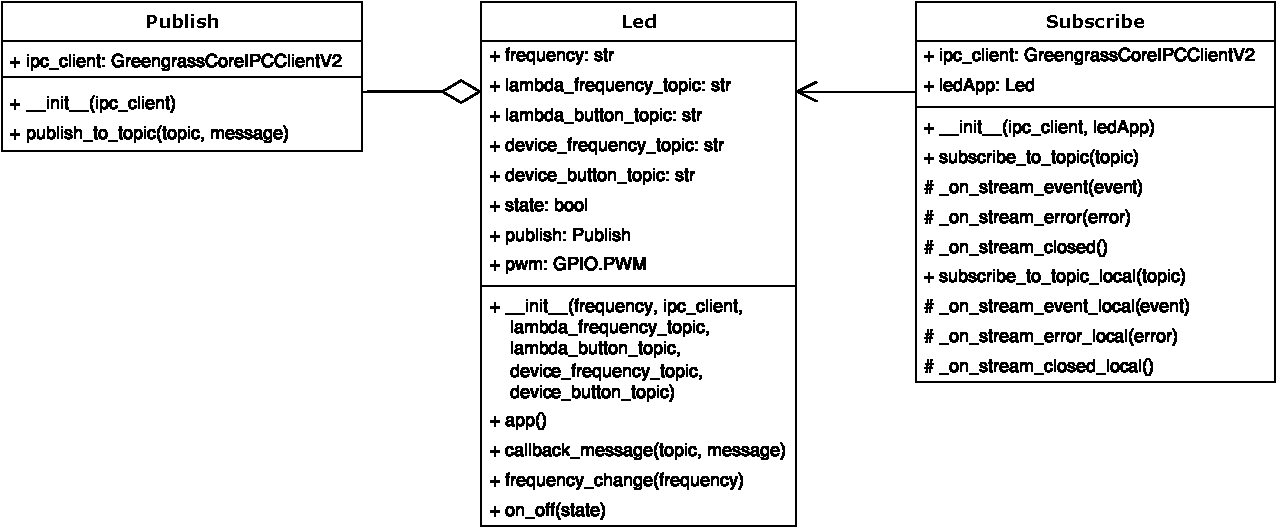
\includegraphics[width=1\columnwidth]{implementation/class_diagram_led_app.pdf}
    \captionof{figure}{Led application class diagram}
    \label{fig:class_diagram_led_app}
    \endgroup
\end{center}
Below is a description of the various classes :
\begin{itemize}
    \item \textit{Led} : Main class that includes the program's main loop. It changes the blinking frequency of the led according to the messages received. It also manages the activation and deactivation of the blinking.
    \item \textit{Publish} : Class that publishes \acrshort{mqtt} messages to \gls{aws} \acrshort{iot}.
    \item \textit{Subscribe} : Class that receives \acrshort{mqtt} messages from \gls{aws} \acrshort{iot} and the button application at local level.
\end{itemize}
The application's behaviour is shown in figure \ref{fig:sequence_diagram_led_app} by a sequence diagram.
\begin{center}
    \begingroup
    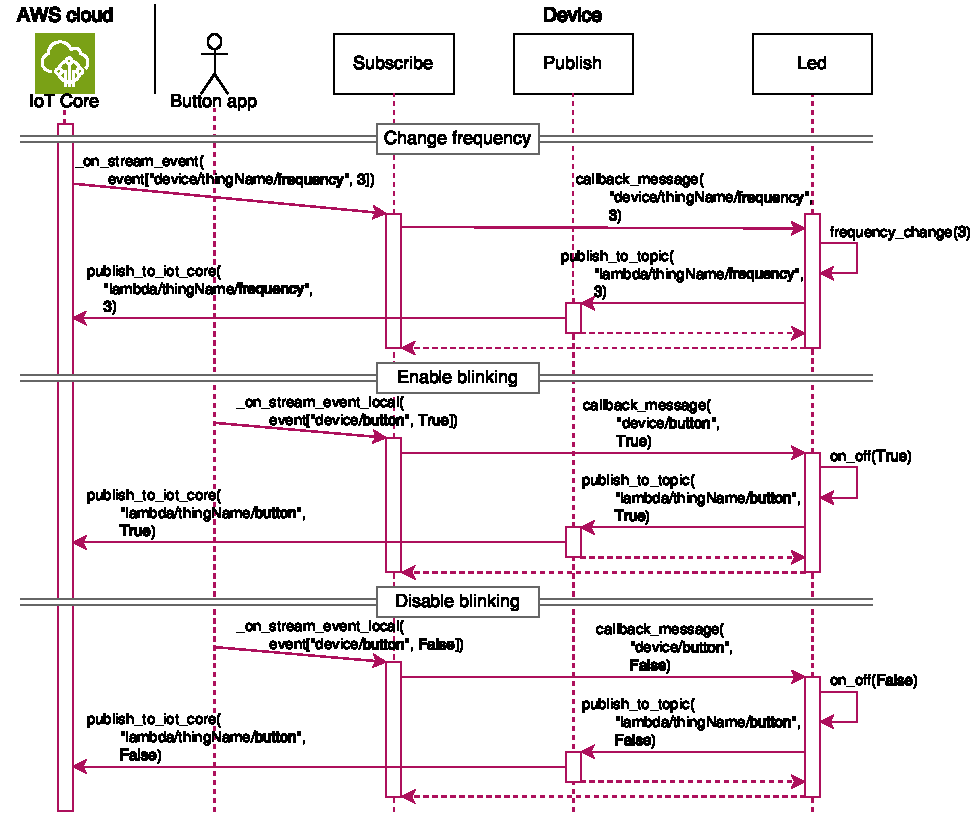
\includegraphics[width=.9\columnwidth]{implementation/sequence_diagram_led_app.pdf}
    \captionof{figure}{Led application sequence diagram}
    \label{fig:sequence_diagram_led_app}
    \endgroup
\end{center}
The frequency is modified from an interface associated with \gls{aws} \acrshort{iot} Core, which sends messages asynchronously. The message is routed to the core class, which responds by sending an \acrshort{mqtt} message to \gls{aws} \acrshort{iot} to confirm receipt and optionally logs this data in an interface. Activation of the blinking is controlled by a button on the device, managed by the button application. Depending on the events, a local \acrshort{mqtt} message is transmitted to the main class. The \textit{Led} class sends a confirmation to \gls{aws} \acrshort{iot} with the status of the blinking, so that it can be logged if necessary. When the external button is pressed a second time, the status is logically reversed.

\subsection{Button application}
The button application has been implemented using the following class diagram \ref{fig:class_diagram_button_app}. The programming language remains Python.
\begin{center}
    \begingroup
    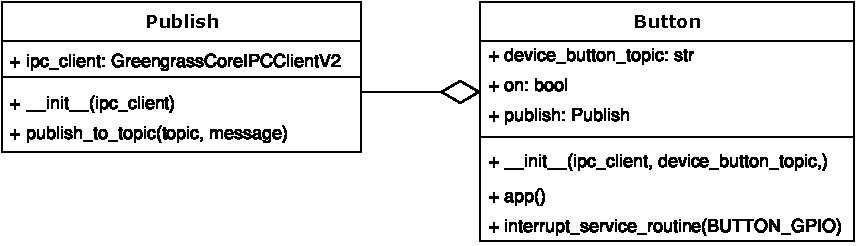
\includegraphics[width=.8\columnwidth]{implementation/class_diagram_button_app.pdf}
    \captionof{figure}{Button application class diagram}
    \label{fig:class_diagram_button_app}
    \endgroup
\end{center}
Here is a description of the different classes :
\begin{itemize}
    \item \textit{Button} : Main class that contains the program's main loop. This is the class that manages the interrupts each time the external button is pressed. \acrshort{mqtt} messages are prepared by this class.
    \item \textit{Publish} : Class which publishes local \acrshort{mqtt} messages to the led application.
\end{itemize}

The sequence diagram \ref{fig:sequence_diagram_button_app} describes the internal workings of the application.
\begin{center}
    \begingroup
    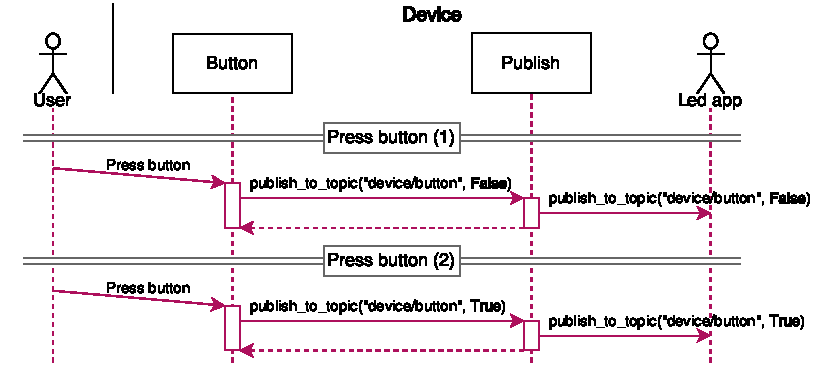
\includegraphics[width=1\columnwidth]{implementation/sequence_diagram_button_app.pdf}
    \captionof{figure}{Button application sequence diagram}
    \label{fig:sequence_diagram_button_app}
    \endgroup
\end{center}
The user can press the external button connected to the \acrshort{iot} device at any time. An interrupt is triggered in the main class, reversing the current state of the blinking. In the sequence diagram scenario, blinking was initially enabled. The first time it is pressed, the blinking is deactivated. An \acrshort{mqtt} message is then sent to the led application. When the button is pressed again, the status is reversed and the blinking should reactivate.

\subsection{Corrupt application}
As mentioned in the section on containerization \ref{sec:containerization}, it is possible to specify the processor architecture on which the Docker container should run. On \nameref{sec:arm_systemready} certified embedded systems, the \gls{arm} processor architecture is \textit{arm64}. To make this application ineligible to run, an incorrect architecture is specified. In this case, the \textit{amd64} architecture has been deliberately specified in the Dockerfile, as follows :
\begin{center}
    \usemintedstyle{pastie}
    \begin{minted}
    [
    fontsize=\scriptsize
    ]{text}
    FROM --platform=linux/amd64 python:latest

    CMD ["echo", "Corrupt Docker container"]
    \end{minted}
\end{center}
The Greengrass component itself is correctly implemented and will run normally. However, when executing the Docker command with the incompatible image, an error occurs.

\subsection{OS update}